%======================================================================================================================% Based on THESIS_WITHOUT_PDFCODE.tex from David.Winterbottom@gmail.com
%======================================================================================================================

%using article instead of report: no need for chapters, only sections
\documentclass[10pt,a4paper]{article}

% Essential packages
\usepackage{amsmath, amssymb, amsthm}
\usepackage{graphicx, color}
\usepackage[top=3cm, bottom=4cm, left=2cm, right=2cm]{geometry}
\usepackage[square, comma, numbers, sort&compress]{natbib}
\usepackage[T1]{fontenc}

% Optional customisation packages
\usepackage{mathpazo}
\usepackage{lineno}
\usepackage{fancyhdr}
\usepackage{lastpage}
\usepackage[hidelinks]{hyperref}

% Page layout
\parindent 0pt
\parskip 1ex
\setlength{\headheight}{40pt}
\setlength{\footskip}{40pt}
\renewcommand{\baselinestretch}{1.33}
\numberwithin{equation}{section}
\renewcommand{\bibname}{References}
\renewcommand{\contentsname}{Contents}
\bibliographystyle{unsrtnat}

%=============================================================================================================================
\newcommand{\fr}[1]{\frac{1}{#1}}

\newcommand{\abs}[1]{\left|#1\right|}
\newcommand{\norm}[1]{\left\Vert#1\right\Vert}

\newcommand{\block}[1]{\left[#1\right]}
\newcommand{\seq}[1]{\left<#1\right>}
\newcommand{\mat}[1]{\left(#1\right)}

\newcommand{\re}[1]{\operatorname{Re}\left(#1\right)}
\newcommand{\im}[1]{\operatorname{Im}\left(#1\right)}

\newcommand{\m}[1]{\mathrm{#1}}

%=============================================================================================================================
\begin{document}
%=============================================================================================================================

%=============================================================================================================================
\begin{titlepage}
%=============================================================================================================================

%Make our own title on an empty page (without footer and header)
%See fancyhdr.pdf
\fancypagestyle{empty}
\lhead{}
\chead{}
\rhead{}
\lfoot{}
\lfoot{}
\cfoot{}
\rfoot{}
\renewcommand{\headrulewidth}{0pt}
\renewcommand{\footrulewidth}{0pt}

\begin{center}
\begin{tabular}{c}
    \Huge{Synthetic Signal Shaping} \\ \\
    \Large{Analytic-gradient phase optimization for target moments and cross-spectral density} \\ \\
    \large{Luc Holtkamp} \\
    \normalsize{SenseMagic, Netherlands} \\
    \normalsize{\texttt{luc@sensemagic.nl}} \\ \\
    % TODO: replace with an original figure generated by the MIMO synthesizer.
    % The former Pollock reproduction (pollock.jpg) is copyright-protected
    % (US: ~2035--2045; EU: public domain 2027) and must not be redistributed.
    % \includegraphics[width=0.9\textwidth]{pollock.jpg} \\ \\
    \vspace{5cm}
\end{tabular}
\end{center}

%=============================================================================================================================
\end{titlepage}
%=============================================================================================================================

\linenumbers

%=============================================================================================================================
\section*{Abstract}
%=============================================================================================================================
We present a phase-domain method for generating multi-input synthetic vibration signals that match a prescribed cross-spectral density (CSD) together with a user-selected set of higher-order diagonal \emph{and joint} moments. The CSD is enforced structurally by pre-multiplying random-phase, unit-modulus, frequency-domain signals with a Cholesky factor of the target CSD, following the frequency-domain synthesis of Shinozuka and Jan~\cite{shinozuka1972digital} and its extensions to partially coherent and non-Gaussian MIMO outputs~\cite{smallwood1993coherent,smallwood_nongaussian,cui2011matrix}. The remaining phase degrees of freedom are used to shape the channelwise moments -- extending the IFFT phase-manipulation idea of Steinwolf~\cite{steinwolf2011ifft,steinwolf2011twr,steinwolf_book_ngaussian} -- and, crucially, also the joint cross-moments (co-skewness, co-kurtosis) which govern coincident-peak excursions and hence multi-axial fatigue damage~\cite{saathoff2006synthetic}. Closed-form analytic gradients of both diagonal and cross moments with respect to the free phases are derived; each cross-moment target of order $m$ (the number of channel indices in the moment) adds at most $m$ FFTs per gradient evaluation, independent of the number of channels. The resulting problem is smooth and is solved with an analytic-gradient sequential-approximation method (CCSAQ~\cite{svanberg2002ccsaq}) from the NLopt library~\cite{johnson_nlopt}. When the target statistics are estimated from measured multi-axial records the targets are realisable by construction, which we argue is the natural regime for the method. Because every target gradient reduces to the same pattern -- one Fourier transform of the pointwise derivative of a memoryless functional, projected through the conjugated unit-modulus source spectrum $u^*$ and the conjugated frequency response $H^*$ -- the MIMO synthesiser inherits the algorithmic simplicity of the single-channel case, and the framework accommodates any smooth memoryless target functional (moments, cross-moments, endpoint values, absolute-value moments, coincident-excursion probabilities, fatigue-dosage surrogates) with no new machinery.

\pagestyle{fancy}
\lhead{ 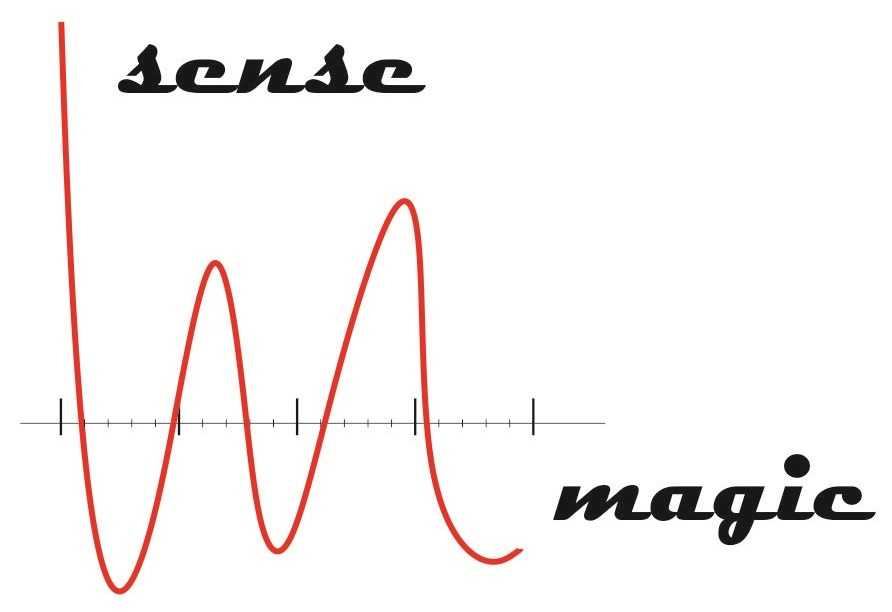
\includegraphics[height=12mm]{SenseMagic.jpg} }
\chead{}
\rhead{\Large Synthetic Signal Shaping \vspace{1mm}}
\lfoot{\parbox[t]{0.6\textwidth}{ \footnotesize
        \textcopyright\ Luc Holtkamp (SenseMagic), 2013--2026. \\
        Licensed under \href{https://creativecommons.org/licenses/by/4.0/}{CC BY 4.0}. \\
        Contact: \texttt{luc@sensemagic.nl} \textbullet\ \texttt{www.sensemagic.nl} }}
\cfoot{}
\rfoot{\parbox[t]{0.3\textwidth} {\footnotesize
		\hfill 
    \begin{tabular}[t]{l l}
        Page:    & \thepage\ of \pageref{LastPage} \\
        File:    &  \jobname \\
        Version: & 0.1
    \end{tabular} }}
\renewcommand{\headrulewidth}{0.5pt}
\renewcommand{\footrulewidth}{0.5pt}


%=============================================================================================================================
\section*{Synthetic signals}
%=============================================================================================================================
The goal is to make a time domain signal with a predefined cross correlation (CSD) and time invariant higher moments.

In the frequency domain we can generate pseudo random noise with a predefined CSD in a simple way, by calculating the complex product of 
a signal with random phase and magnitude one and a matrix $\mathbf{H}$ defined by $\mathbf{H}^*\mathbf{H} = \mathbf{G}$, where $\mathbf{G}$ is the target CSD. 
$\mathbf{H}$ can be calculated with the Cholesky decomposition~\cite{shinozuka1972digital,smallwood1993coherent}.

%=============================================================================================================================
\section*{Related work and positioning}
%=============================================================================================================================

Frequency-domain synthesis of stationary Gaussian random processes with a prescribed spectrum dates back to Rice~\cite{rice1944mathematical} and was cast in its modern digital form by Shinozuka and Jan~\cite{shinozuka1972digital}. The MIMO extension -- pre-multiplying random-phase spectra with a Cholesky factor of the target CSD -- is due to Smallwood and Paez~\cite{smallwood1993coherent}, with follow-on work on partially coherent and non-Gaussian outputs~\cite{smallwood_nongaussian,cui2011matrix,hsueh1990generalized}. This structural approach is now the standard basis of MIMO random-vibration controllers.

Non-Gaussian shaping falls into two broad families. \emph{Amplitude-domain warping} transforms a Gaussian signal through a memoryless nonlinearity chosen to hit a target skew/kurtosis; the Hermite polynomial transform of Winterstein~\cite{winterstein1988nonlinear} is the canonical example. It is simple and closed-form but distorts the spectrum. \emph{Phase manipulation} keeps $|U(f)|$ fixed and manipulates $\arg U(f)$ so that the moments of the inverse-FFT time signal reach the target, leaving the (auto-)spectrum invariant by construction. The IFFT phase-manipulation method of Steinwolf~\cite{steinwolf2011ifft,steinwolf2011twr,steinwolf_book_ngaussian} is the closest prior art to the present work and is single-channel; extensions to multi-axial excitation with a synthetic road profile appear in Saathoff \emph{et al.}~\cite{saathoff2006synthetic}. The present paper generalises Steinwolf's construction to full MIMO with prescribed CSD, adds \emph{joint} cross-moments (co-skewness, co-kurtosis) to the target set, and provides closed-form analytic gradients for gradient-based optimisation. The phase-only, magnitude-fixed nature of the problem also places it in the broad family of phase-retrieval algorithms~\cite{gerchberg1972practical,fienup1982phase}, although here the constraint set is on time-domain moments rather than on a second image plane.

Related nonlinear-identification techniques (Volterra series, parallel cascades, block-oriented models) and their use inside iterative test-control loops~\cite{bendat1998nonlinear,pintelon_schoukens_ident,schoukens_odd_multisine} motivate the multi-axial setup but are not the subject of this paper; a companion note develops that connection separately. The framework presented here is not a purely academic construction: variants of it have been deployed by the author in several industrial projects for customers, in particular for model-estimation campaigns driven by minimum-kurtosis excitation, where concentrating the available actuator headroom into a dense, low-crest drive signal maximises the signal-to-noise ratio of the estimated response models.

%=============================================================================================================================
\section*{Definitions of signals and moments}
%=============================================================================================================================

Let the signal $\mathbf{u}$ a complex variable in the frequency domain with $N_j$ channels. The signal $\mathbf{v}$ is the result of filtering $\mathbf{u}$ with the complex frequency response funcion $\mathbf{H}$ with magnitude $\mathbf{h}$ and phase $\theta$.

The result signal in the time domain is the channel wise inverse Fourier transform of $\mathbf{v}$.

\begin{eqnarray}
	H_{k j f} &=& h_{k j f} \: \m{e}^{\m{i} \theta_{k j f}} \\
	u_{k f} &=& \m{e}^{\m{i} \psi_{k f}} \\
	v_{k f} &=& \sum_{j=0}^{N_j-1} H_{k j f} \; \m{e}^{\m{i} \psi_{j f}} 
			\;=\; \sum_{j=0}^{N_j-1} h_{k j f} \: \m{e}^{\m{i} \theta_{k j f}} \:\; \m{e}^{\m{i} \psi_{j f}} \\
	\mathbf{x_k} &=& \mathcal{F}^{\m{-1}} \mat{\mathbf{v_k}}
\end{eqnarray}
Assume further that $\mathbf{x}$ has $N_t$ samples. We can then expand $x_t$ as:
\begin{eqnarray}
	x_{k t}
	&=& \mathcal{F}^{\m{-1}}_t \mat{\mathbf{v_k}} \\
	&=&  \frac{1}{N_t} \sum_{f=0}^{N_t-1}
\sum_{j=0}^{N_j-1} h_{k j f} \; \m{e}^{\m{i}\mat{\frac{2 \pi t f}{N_t} + \theta_{k j f} + \psi_{j f}}} 
\end{eqnarray}
We will require that $\mathbf{x}$ is real and has zero mean and zero energy at the Nyquist frequency (the latter is both a mathematical convenience and a physical necessity, discussed in the subsection on logical vs physical moments below), which means that for $1 \leq f < Nt/2$
\begin{eqnarray}
	\theta_{k j f} &=& - \theta_{k j \mat{N_t  - f}} \\
	h_{k j f} &=& h_{k j \mat{N_t  - f}} \\
	\psi_{j f} &=& - \psi_{j \mat{N_t  - f}}
\end{eqnarray}
Which means that we can write for $\mathbf{x}$:
\begin{eqnarray}
	x_{k t}
	&=&  \frac{1}{N_t} \sum_{f=0}^{N_t-1}
		\sum_{j=0}^{N_j-1} h_{k j f} \; \m{e}^{\m{i}\mat{\frac{2 \pi t f}{N_t} + \theta_{k j f} + \psi_{j f}}} \\
	&=&  \frac{1}{N_t} \sum_{f=1}^{N_t/2-1}
		\sum_{j=0}^{N_j-1} 
		\mat{h_{k j f} \; \m{e}^{\m{i}\mat{\frac{2 \pi t f}{N_t} + \theta_{k j f} + \psi_{j f}}}			
		+ h_{k j \mat{N_t - f}} \; \m{e}^{\m{i}\mat{\frac{2 \pi t \mat{N_t - f}}{N_t} + \theta_{k j \mat{N_t - f}} + \psi_{j \mat{N_t - f}}}}} \\
	&=&  \frac{1}{N_t} \sum_{f=1}^{N_t/2 - 1}
		\sum_{j=0}^{N_j-1} 
		\mat{h_{k j f} \; \m{e}^{\m{i}\mat{\frac{2 \pi t f}{N_t} + \theta_{k j f} + \psi_{j f}}}
	    + h_{k j f} \; \m{e}^{-\m{i}\mat{\frac{2 \pi t f}{N_t} + \theta_{k j f} + \psi_{j f}}}} \\	
	&=&	\frac{2}{N_t} \sum_{f=1}^{N_t/2 - 1}
		\sum_{j=0}^{N_j-1} h_{k j f} \; \cos\mat{\frac{2 \pi t f}{N_t} + \theta_{k j f} + \psi_{j f}} \\
\end{eqnarray}
Now define, for any ordered tuple of channel indices $\mathbf{i} = \mat{i_1,\ldots,i_m}$ with entries in $\block{0,\ldots,N_j-1}$ and length $|\mathbf{i}|=m\geq 1$, the raw joint moment
\begin{eqnarray}
P_\mathbf{i} &=& \frac{1}{N_t}\sum_{t=0}^{N_t-1} \prod_{a=1}^{m} x_{i_a, t}.
\end{eqnarray}
The tuple $\mathbf{i} = k^{(m)} \equiv \mat{\underbrace{k,\ldots,k}_{m}}$ recovers the channelwise diagonal moment $P_{k^{(m)}} = \frac{1}{N_t}\sum_t x_{k,t}^m$; the tuple $(k,k)$ gives the channel variance $P_{(k,k)}$; and $(i,j)$ with $i\neq j$ gives the time-averaged cross-covariance. The second-order tuples are fixed structurally by the CSD constraint through $\mathbf{H}$ and are therefore excluded from the target set below.

The normalised joint moment is
\begin{eqnarray}
M_\mathbf{i} &=& \frac{P_\mathbf{i}}{\prod_{a=1}^{m} \sqrt{P_{\mat{i_a,i_a}}}} \qquad \mat{m \geq 3},
\end{eqnarray}
with the convention $M_{(k)} = 0$ (zero-mean constraint). Special cases: $M_{k^{(3)}}$ is the channelwise skewness, $M_{k^{(4)}}$ the channelwise kurtosis, $M_{(i,j,k)}$ with distinct indices a \emph{co-skewness}, and $M_{(i,i,j,j)}$ a \emph{co-kurtosis} -- the latter governing coincident-peak behaviour and hence multi-axial fatigue damage~\cite{saathoff2006synthetic}. Steinwolf's original construction~\cite{steinwolf2011ifft} shapes $M_{k^{(3)}}$ and $M_{k^{(4)}}$ only; the added value of the present formulation is the joint-index case.

%=============================================================================================================================
\subsection*{The loss function}
%=============================================================================================================================
The target set $\mathcal{S}$ is a user-selected collection of tuples with $|\mathbf{i}|\geq 3$, each carrying a target value $\mu_\mathbf{i}$ and optional weight $w_\mathbf{i}$. Typical choices include the diagonal tuples $\seq{k^{(3)},\,k^{(4)}:\,k=0,\ldots,N_j-1}$ for per-channel skew and kurtosis, and the cross tuples $\seq{(i,i,j,j):\,i<j}$ for pair co-kurtoses. The loss is the weighted sum of squared deviations
\begin{eqnarray}
\Xi &=& \frac{1}{2}\sum_{\mathbf{i}\in\mathcal{S}} w_\mathbf{i}\,\mat{M_\mathbf{i} - \mu_\mathbf{i}}^2.
\end{eqnarray}

%=============================================================================================================================
\subsection*{Gradient of the loss}
%=============================================================================================================================
By the chain rule,
\begin{eqnarray}
\frac{\partial \Xi}{\partial \psi_{q g}} &=& \sum_{\mathbf{i}\in\mathcal{S}} w_\mathbf{i}\,\mat{M_\mathbf{i} - \mu_\mathbf{i}}\,\frac{\partial M_\mathbf{i}}{\partial \psi_{q g}},
\end{eqnarray}
so we need $\partial M_\mathbf{i}/\partial \psi_{q g}$, which in turn depends on $\partial P_\mathbf{i}/\partial \psi_{q g}$ and $\partial P_{(i_a,i_a)}/\partial \psi_{q g}$. All of these are instances of a single observation, which we state first and then apply.

\textbf{Key observation.} Let $g:\mathbb{R}^m\to\mathbb{R}$ be any per-sample memoryless differentiable functional and consider the time-averaged target
\begin{eqnarray}
Q\mat{\mathbf{x}} &=& \frac{1}{N_t}\sum_{t=0}^{N_t-1} g\mat{x_{i_1, t},\, x_{i_2, t},\, \ldots,\, x_{i_m, t}}.
\end{eqnarray}
Using $\partial x_{k,t}/\partial \psi_{q g} = -\frac{2}{N_t}\, h_{k q g}\sin\mat{\frac{2 \pi t g}{N_t} + \theta_{k q g} + \psi_{q g}}$ and the chain rule,
\begin{eqnarray}
\frac{\partial Q}{\partial \psi_{q g}}
	&=& \frac{1}{N_t}\sum_{t=0}^{N_t-1}\sum_{a=1}^{m}\mat{\partial_a g}\mat{x_{i_1,t},\ldots,x_{i_m,t}}\,\frac{\partial x_{i_a,t}}{\partial \psi_{q g}} \\
	&=& -\frac{2}{N_t^2}\sum_{a=1}^{m}\sum_{t=0}^{N_t-1}\mat{\partial_a g}\mat{x_{i_1,t},\ldots,x_{i_m,t}}\; h_{i_a q g}\,\sin\mat{\frac{2 \pi t g}{N_t} + \theta_{i_a q g} + \psi_{q g}}.
\end{eqnarray}
Writing $\sin z = \im{\m{e}^{\m{i} z}}$ and collecting the phase factors as $h_{i_a q g}\,\m{e}^{\m{i}\theta_{i_a q g}} = H_{i_a q g}$ and $\m{e}^{\m{i}\psi_{q g}} = u_{q g}$,
\begin{eqnarray}
\frac{\partial Q}{\partial \psi_{q g}}
	&=& -\frac{2}{N_t^2}\;\im{u_{q g} \sum_{a=1}^{m} H_{i_a q g} \sum_{t=0}^{N_t-1}\mat{\partial_a g}\mat{x_{i_1,t},\ldots,x_{i_m,t}}\;\m{e}^{\m{i}\frac{2 \pi t g}{N_t}}}.
\end{eqnarray}
The inner sum over $t$ is the complex conjugate of the forward Fourier transform $\mathcal{F}_g\block{y} = \sum_t y_t\,\m{e}^{-\m{i} 2\pi t g/N_t}$ evaluated on the real sequence $\mat{\partial_a g}_t$; conjugating the whole argument and using $\im{z^*} = -\im{z}$ gives
\begin{eqnarray}
\frac{\partial Q}{\partial \psi_{q g}}
	&=& \frac{2}{N_t^2}\;\im{u_{q g}^* \sum_{a=1}^{m} H_{i_a q g}^*\;\mathcal{F}_g\block{\mat{\partial_a g}\mat{x_{i_1,\cdot},\ldots,x_{i_m,\cdot}}}}.
\end{eqnarray}
\emph{The phase-gradient of any memoryless functional of the inverse-Fourier signal is itself a Fourier transform} -- specifically, of the pointwise partial derivative $\partial_a g$ with respect to the $a$-th argument, projected through $u_{q g}^*$ and $H_{i_a q g}^*$ and averaged over the arguments $a=1,\ldots,m$. One FFT per distinct argument of $g$ suffices; repeated arguments share their FFT. Every target-gradient in the paper is an instance of this identity, so the optimiser needs only two building blocks: the pointwise derivatives $\partial_a g$, and one length-$N_t$ FFT of each.

\textbf{Instance: joint moments.} With $g\mat{y_1,\ldots,y_m} = \prod_{a=1}^{m} y_a$, so $\partial_a g = \prod_{b\neq a} y_b$, the observation gives
\begin{eqnarray}
\frac{\partial P_\mathbf{i}}{\partial \psi_{q g}}
	&=& \frac{2}{N_t^2}\;\im{u_{q g}^* \sum_{a=1}^{m} H_{i_a q g}^*\;\mathcal{F}_g\block{\prod_{b\neq a} x_{i_b,\cdot}}}.
\end{eqnarray}

\textbf{Instance: diagonal moment.} For $\mathbf{i} = k^{(m)}$ all $m$ partial products equal $x_{k,\cdot}^{m-1}$ and all $m$ frequency factors equal $H_{k q g}^*$, so
\begin{eqnarray}
\frac{\partial P_{k^{(m)}}}{\partial \psi_{q g}} &=& \frac{2 m}{N_t^2}\,\im{u_{q g}^*\, H_{k q g}^*\;\mathcal{F}_g\block{x_{k,\cdot}^{m-1}}},
\end{eqnarray}
recovering the single-channel Steinwolf-style gradient~\cite{steinwolf2011ifft} as a special case.

\textbf{Instance: co-skewness.} For $\mathbf{i}=(i,j,k)$ with distinct entries,
\begin{eqnarray}
\frac{\partial P_{(i,j,k)}}{\partial \psi_{q g}} &=& \frac{2}{N_t^2}\;\im{u_{q g}^*\block{H_{i q g}^*\,\mathcal{F}_g\block{x_j x_k} + H_{j q g}^*\,\mathcal{F}_g\block{x_i x_k} + H_{k q g}^*\,\mathcal{F}_g\block{x_i x_j}}}.
\end{eqnarray}

\textbf{Instance: co-kurtosis.} For $\mathbf{i}=(i,i,j,j)$ the partial products collapse pairwise so only two FFTs are needed:
\begin{eqnarray}
\frac{\partial P_{(i,i,j,j)}}{\partial \psi_{q g}} &=& \frac{4}{N_t^2}\;\im{u_{q g}^*\block{H_{i q g}^*\,\mathcal{F}_g\block{x_i x_j^2} + H_{j q g}^*\,\mathcal{F}_g\block{x_j x_i^2}}}.
\end{eqnarray}

\textbf{Instance: variance.} Taking $g\mat{y} = y^2$ so $\partial_y g = 2 y$, and using $\mathcal{F}_g\block{x_{k,\cdot}} = v_{k g}$,
\begin{eqnarray}
\frac{\partial P_{(k,k)}}{\partial \psi_{q g}}
	&=& \frac{4}{N_t^2}\,\im{u_{q g}^*\, H_{k q g}^*\;\mathcal{F}_g\block{x_{k,\cdot}}}
	\;=\; \frac{4}{N_t^2}\,\im{u_{q g}^*\, H_{k q g}^*\, v_{k g}}.
\end{eqnarray}
The $v_{k g}$ are computed once at the start of every iteration (they are needed to obtain $x_{k,t}$ in the first place), so the variance gradient is free.

\textbf{Chain rule on the normalisation.}
\begin{eqnarray}
\frac{\partial M_\mathbf{i}}{\partial \psi_{q g}}
	&=& \frac{1}{\prod_{a=1}^{m}\sqrt{P_{(i_a,i_a)}}}
	\block{\frac{\partial P_\mathbf{i}}{\partial \psi_{q g}}
	- \frac{P_\mathbf{i}}{2}\sum_{a=1}^{m}\frac{1}{P_{(i_a,i_a)}}\frac{\partial P_{(i_a,i_a)}}{\partial \psi_{q g}}}.
\end{eqnarray}

\textbf{Remark: MIMO is more of the same.} In the single-channel case the per-channel variance $P_{(k,k)}$ is invariant under changes of its own phases (a direct consequence of the FFT identity, or equivalently of $\im{|H_{q q g}u_{q g}|^2}=0$ when $H$ is diagonal), so it factors out of the loss gradient cleanly. In the MIMO case with off-diagonal $H_{p q g}$ the variance of channel $k$ does depend on the phases of other channels through the cross-coupling, and no longer factors out. This looked forbidding when we first attempted the extension, but the key observation dissolves the concern: the variance derivative is itself an instance of the same FFT identity, and its contribution to the total gradient is one already-computed pass ($v_{k g}$) per channel. Every additional target -- diagonal moment, cross-moment, variance, endpoint value, or any user-supplied smooth memoryless functional -- adds at most $|\mathbf{i}|$ FFTs to the iteration and nothing conceptually new.

\textbf{Cost.} Each target tuple contributes at most $|\mathbf{i}|$ length-$N_t$ FFTs to the gradient (fewer when partial products repeat). The variance passes $v_{k g}$ needed for normalisation are shared across all targets referencing channel $k$; one pass per channel suffices per iteration. For $N_j$ output channels with all per-channel skew/kurtosis plus all pair co-kurtoses in $\mathcal{S}$, the per-iteration FFT count is $O\mat{N_j^2}$ -- negligible compared to the informational gain from constraining the joint distribution.

\textbf{Feasibility.} When the target statistics $\mu_\mathbf{i}$ are estimated from a measured multi-channel record (see the multitaper subsection below), they are realisable by construction and the optimiser converges to a signal matching them within the ill-posedness of a finite block length. For analytically prescribed targets, no closed-form realisability bounds are known in the general case; we recommend a pre-check that evaluates $M_\mathbf{i}$ at the random-phase initialisation and flags targets lying more than a few standard deviations away from that ensemble.

\textbf{Beyond polynomial moments.} Because the key observation places no restriction on $g$ beyond memorylessness and differentiability, any smooth functional of the signal is a legitimate target for the same optimiser without new machinery: absolute-value moments $g\mat{y}=|y|^m$ (with the sign function as $\partial_a g$), smooth surrogates for peak counts and sign-crossings, coincident-excursion probabilities via smoothed indicator products, and fatigue-dosage functionals of the rainflow-count form when a differentiable surrogate is supplied. The user provides $g$ and $\partial_a g$ as pointwise functions; the optimiser handles the rest.

%=============================================================================================================================
\subsection*{Endpoint continuity for streamed blocks}
%=============================================================================================================================

Two common use cases require control over block boundaries: (i) \emph{periodic FRF estimation}, where a single block is repeated $N$ times and the first $M$ repetitions are discarded so the response settles into a periodic steady state before averaging; and (ii) \emph{live streaming}, where independent blocks -- each with fresh random phases -- are concatenated on the fly for extended shaker runs.

\textbf{Case (i) is free of seam artefacts, but not of start-up ones.} The inverse-FFT signal is periodic with period $N_t$ by construction: $x_{k, N_t} = x_{k, 0}$ and the derivative is likewise periodic. Repeating one block produces a smooth concatenation on the ring $\mathbb{Z}/N_t\mathbb{Z}$; the transient observed at the test rig is entirely the plant's response to a periodic input, which is exactly what one wishes to average out. In practice, however, the \emph{first} block still starts from rest, and an arbitrary head value $x_{k,0}$ produces an initial discontinuity when the drive is switched on. One therefore still wants a defined start value (typically zero) together with a short fade-in taper on the first repetition -- so the endpoint constraint of case (ii) below is useful here too, even though the repetitions themselves splice exactly.

\textbf{Case (ii) requires a fringe constraint.} Successive blocks $B$ and $B{+}1$ share their seam at $t=N_t \equiv 0$. Unless $x^{B+1}_{k, 0} = x^{B}_{k, N_t} \equiv x^{B}_{k, 0}$ (and the analogous condition on the slope) the stream has a jump or a slope kink at every block boundary, showing up in the effective spectrum as broadband leakage. The synthesiser fixes the block's head value and slope to prescribed constants $c^{(0)}_k$, $c^{(1)}_k$ for every block; consecutive blocks then splice with $C^1$ continuity by construction. Zero is the natural default and is used throughout the reference implementation, giving a signal that starts and returns to rest at every block boundary.

The head value and its time derivative follow directly from the cosine expansion of $x_{k,t}$:
\begin{eqnarray}
x_{k, 0}      &=& \frac{2}{N_t}\sum_{f=1}^{N_t/2-1}\sum_{j=0}^{N_j-1} h_{k j f}\,\cos\mat{\theta_{k j f}+\psi_{j f}}
	\;=\; \frac{2}{N_t}\sum_{f,j}\re{H_{k j f}\, u_{j f}}, \\
\dot x_{k, 0} &=& -\frac{2}{N_t}\sum_{f=1}^{N_t/2-1}\sum_{j=0}^{N_j-1}\omega_f\,h_{k j f}\,\sin\mat{\theta_{k j f}+\psi_{j f}}
	\;=\; -\frac{2}{N_t}\sum_{f,j}\omega_f\,\im{H_{k j f}\, u_{j f}},
\end{eqnarray}
with $\omega_f = 2\pi f / N_t$. The synthesiser adds the endpoint terms to the loss,
\begin{eqnarray}
\Xi_{\m{ep}} &=& \frac{1}{2}\sum_{k=0}^{N_j-1}\block{w^{(0)}_k\mat{x_{k, 0} - c^{(0)}_k}^2 + w^{(1)}_k\mat{\dot x_{k, 0} - c^{(1)}_k}^2},
\end{eqnarray}
and the gradients follow immediately:
\begin{eqnarray}
\frac{\partial x_{k, 0}}{\partial \psi_{q g}}      &=& -\frac{2}{N_t}\,\im{H_{k q g}\, u_{q g}}, \\
\frac{\partial \dot x_{k, 0}}{\partial \psi_{q g}} &=& -\frac{2\omega_g}{N_t}\,\re{H_{k q g}\, u_{q g}}.
\end{eqnarray}
No additional FFT is required: the endpoint contribution to the total gradient is a single complex multiply--add per $(q,g)$ per constrained channel. This is the degenerate case of the key observation with the sample-average replaced by point evaluation at $t{=}0$; the ``FFT of the pointwise gradient'' collapses to a Kronecker delta and evaluates trivially. Constraining the block's tail is redundant given the block's built-in periodicity and given that fixing every block's head simultaneously fixes the tail to which each previous block will connect.

The endpoint constraint removes $2 N_j$ degrees of freedom from the $N_j\mat{N_t/2-1}$-dimensional phase space -- a fraction that vanishes as $N_t\to\infty$ -- and so interacts benignly with the moment targets at any practically useful block length.

%=============================================================================================================================
\subsection*{Direct minimisation: a smooth crest-factor surrogate}
%=============================================================================================================================

For model estimation and endurance testing one often wants the \emph{opposite} of heavy tails: minimum kurtosis and minimum crest factor $\max_t\abs{x_{k t}}/s_k$ (with $s_k = \sqrt{P_{(k,k)}}$), concentrating the signal energy and maximising the drive level attainable within actuator limits. The crest factor itself is a poor optimisation objective: its gradient is supported only at the extremal sample, so a gradient step relocates the peak elsewhere in the block and the optimiser hops between candidate peaks without converging. Minimising the kurtosis $M_{k^{(4)}}$ instead is smooth but weights peaks only polynomially and stalls at a crest well above the achievable floor; higher even moments ($M_{k^{(8)}}$, $M_{k^{(16)}}$) push further but exhibit the same plateau behaviour.

A smooth surrogate with \emph{exponential} peak weighting resolves this. For channel $k$ define
\begin{eqnarray}
\Xi_{\m{crest}} &=& \frac{w}{\beta}\,\ln\mat{\frac{1}{N_t}\sum_{t=0}^{N_t-1}\cosh z_{k t}},
\qquad z_{k t} \;=\; \frac{\beta\, x_{k t}}{s_k},
\end{eqnarray}
which approaches $w \max_t \abs{x_{k t}}/s_k$ from below as $\beta\to\infty$, with bias of order $\ln\mat{2 N_t}/\beta$. This term is added directly to the loss (it has no target value) and its gradient is one more instance of the key observation: with $C = \frac{1}{N_t}\sum_t \cosh z_{k t}$,
\begin{eqnarray}
\frac{\partial \Xi_{\m{crest}}}{\partial \psi_{q g}}
	&=& \frac{w}{C}\block{\frac{1}{s_k}\,\frac{2}{N_t^2}\,\im{u_{q g}^*\, H_{k q g}^*\;\mathcal{F}_g\block{\sinh z_{k,\cdot}}}
	- \frac{1}{2 s_k^3}\mat{\frac{1}{N_t}\sum_t x_{k t}\sinh z_{k t}}\frac{\partial P_{(k,k)}}{\partial \psi_{q g}}},
\end{eqnarray}
one FFT for the memoryless factor $\sinh z$ plus the already-computed variance gradient; the second term is required because in the MIMO case the normalisation $s_k$ depends on the phases of all channels through the off-diagonal $H$. Numerically the surrogate is evaluated in shifted-exponential form ($\cosh$ and $\sinh$ scaled by $\m{e}^{-\max_t\abs{z_{k t}}}$) so that large $\beta$ does not overflow.

Large $\beta$ makes the landscape stiff, and starting a high-$\beta$ optimisation from random phases stalls at a mediocre crest. A \emph{$\beta$-continuation} resolves this at negligible cost: optimise at a small $\beta$, then double $\beta$ and warm-start from the previous optimum. Each stage after the first converges in a small fraction of the initial stage's iterations, and the continuation consistently reaches lower crest factors than any single-stage run of whatever budget (see the example below). The staging mirrors classical $p$-norm continuation for Chebyshev-type problems; the surrogate keeps every stage smooth with analytic gradients.

%=============================================================================================================================
\subsection*{Logical vs physical moments: a Nyquist-tail caveat}
%=============================================================================================================================

The moments $P_\mathbf{i}$ and $M_\mathbf{i}$ shaped by the optimiser are moments of the discrete signal $x_{k, t}$ evaluated on the sample grid $t = 0,\ldots,N_t-1$. This is a deliberate departure from Steinwolf's formulation~\cite{steinwolf2011ifft,steinwolf_book_ngaussian}, which evaluates the kurtosis on the \emph{continuous} periodic inverse Fourier reconstruction; the present method works entirely with the discrete periodic FFT sequence, and the distinction matters for the reasons developed in this subsection. The signal that physically reaches the device under test is the continuous-time reconstruction $x_k\mat{\tau}$ produced by the DAC and its analog reconstruction filter. These two signals coincide asymptotically as spectral content is pushed below Nyquist, but diverge for content that approaches Nyquist -- and the divergence can be substantial.

A single-line example makes this concrete. Let $x_k$ have all its energy in one spectral bin $f_0$ with amplitude $A$. The physical continuous-time signal is a sinewave with kurtosis $M_{k^{(4)}, \m{phys}} = 3/2$ regardless of $f_0$. The sampled sequence, however, is $A\cos\mat{2\pi t f_0/N_t + \psi}$ with $t\in\seq{0,\ldots,N_t-1}$; for $f_0 \ll N_t/2$ this samples the sine densely and the sample-moment kurtosis $M_{k^{(4)}} \to 3/2$, but as $f_0 \to N_t/2$ the sampled sequence becomes the two-valued alternation $\block{+A, -A, +A, -A, \ldots}$ whose sample-moment kurtosis is $1$. The worst-case discrete-versus-physical mismatch is a full ${\approx}33\%$ in kurtosis, achieved precisely at Nyquist.

This is the engineering reason for the requirement $h_{k j,\, N_t/2} = 0$ imposed at the outset: no realisable reconstruction filter can pass content at the Nyquist bin cleanly, so any energy the optimiser placed there would be physically distorted by the analog path before reaching the plant, and the sample-domain moment computed there does not correspond to any physical reality. Setting the Nyquist bin to zero is thus both a mathematical convenience -- it removes a special-case real-only frequency bin from the cosine expansion -- and a physical necessity for any signal that will be played out through a DAC. In practice we go further and assign zero target CSD above a comfortable guard band (typically $\lesssim 0.4\, f_s$), which keeps the Nyquist-tail moment error below ${\sim}1\%$ for spectra of practical interest.

Two operating regimes result. In the \emph{measured-target regime} the mismatch is benign by cancellation: target moments are sample moments of an ADC record, and the synthesiser produces sample moments of the same statistical character. If the measurement ADC and the playback DAC use the same sample rate and comparable anti-alias / reconstruction filtering, the Nyquist-tail distortion is applied identically on both sides and cancels; the physical playback then matches the physical original in moment even though the intermediate quantities being matched live in the sampled domain. This is exactly the practical outcome the end user cares about. In the \emph{analytic-target regime} the user specifies $\mu_\mathbf{i}$ from theory or a spec, and should either band-limit the target CSD as above, or interpret the shaped moments as digital-domain quantities that the digital controller consumes directly -- a legitimate interpretation, since the controller sees the sampled signal and most plant dynamics of practical interest live well below Nyquist.

A related linear effect -- the $|\m{sinc}\mat{f/f_s}|$ amplitude taper of a zero-order-hold DAC together with the amplitude response of the analog reconstruction and anti-alias filters -- distorts the delivered $|H\mat{f}|$ and hence downstream physical moments even in the measured-target regime. This is a rig-integration matter, handled either by compensating in the reconstruction filter or by pre-shaping $H$; it is outside the scope of the synthesiser proper.

%=============================================================================================================================
\subsection*{Estimating targets from measured data}
%=============================================================================================================================

The synthesiser requires a target CSD $\mathbf{G}\mat{f}$ (which determines $\mathbf{H}$ via Cholesky) and a set of higher-order moment targets $\seq{\mu_\mathbf{i}}_{\mathbf{i}\in\mathcal{S}}$. When these are estimated from a measured multi-axial record -- the natural regime for this method -- the choice of estimator matters, because a biased or non-PSD CSD estimate contaminates the Cholesky factor and propagates structurally into every synthesised block.

\textbf{Why not the periodogram or Welch.} The single-taper periodogram has bias controlled by the window's spectral leakage: rectangular windows leak wildly, Hann or Hamming tapers reduce leakage at the cost of resolution but still concentrate all estimator energy on a single window. Welch averaging reduces variance at the cost of frequency resolution and, on records with large dynamic range across frequencies, introduces persistent leakage bias that cannot be averaged out. For cross-spectra the situation is worse: the coherence estimate acquires a positive bias that vanishes only asymptotically.

\textbf{Multitaper with Slepian sequences.} The Thomson multitaper estimator~\cite{thomson1982multitaper} replaces the single window with a family of $K$ orthonormal tapers whose energy is maximally concentrated in a chosen bandwidth $\block{-W, W}$. These tapers are the discrete prolate spheroidal sequences (DPSS) of Slepian~\cite{slepian1978dpss}; the first $K \approx 2 N_t W - 1$ are effectively leakage-free. The multitaper CSD estimate for channels $p,q$ is
\begin{eqnarray}
\hat G_{p q}\mat{f} &=& \frac{1}{K}\sum_{k=0}^{K-1} Y^{(k)}_{p}\mat{f}\; {Y^{(k)}_{q}\mat{f}}^*, \qquad Y^{(k)}_{p}\mat{f} = \mathcal{F}\block{w^{(k)}_t\, y_{p, t}},
\end{eqnarray}
where $w^{(k)}$ is the $k$-th DPSS taper and $y_{p, t}$ is the measured record on channel~$p$. The estimator has approximately $2K$ degrees of freedom, low bias by design, and is manifestly Hermitian positive semi-definite because it is an average of rank-one outer products. Percival and Walden~\cite{percival_walden_1993} give the standard univariate treatment; Walden~\cite{walden2000multivariate} extends it to the MIMO case with jackknife error bars on cross-spectral phase and coherence.

The PSD property is important here: Cholesky factorisation $\mathbf{G}\mat{f} = \mathbf{H}^*\mathbf{H}$ requires $\hat{\mathbf{G}}\mat{f}$ to be PSD at every frequency bin. Estimators that are not manifestly PSD -- windowed cross-periodograms, some parametric schemes, ad-hoc coherence-weighted spectra -- require a projection onto the PSD cone before Cholesky~\cite{higham1988nearest}, which introduces its own bias. The multitaper estimator sidesteps this entirely.

\textbf{Higher-order targets.} The moment targets $\mu_\mathbf{i}$ are estimated directly from the record as sample statistics $\hat P_\mathbf{i} = \frac{1}{N_t}\sum_t \prod_a y_{i_a, t}$, with the corresponding normalisation. Their variance decreases as $1/N_t$ for stationary records; in practice we recommend segmenting a long record and averaging the per-segment $\hat P_\mathbf{i}$, or bootstrapping from the multitaper eigencoefficients as in Percival and Walden~\cite{percival_walden_1993}.

\textbf{Non-stationary records and the multimodel approach.} Measured field records are rarely stationary over their full length. The practical remedy is to partition the record into segments with similar statistics, group those segments, and estimate one CSD-plus-moment target set per group -- yielding a small library of models rather than a single compromise model. The multitaper estimator is particularly well suited to this regime: its low variance per short segment (${\approx}2K$ degrees of freedom from a single block) makes reliable per-group estimates possible where Welch averaging would demand data lengths the group does not have. Synthesis then proceeds per model, and the models can be sequenced or blended to reproduce the non-stationary character of the original environment. We have found this \emph{multimodel} approach promising in practice; a companion note, with worked examples, will develop it separately.

%=============================================================================================================================
\section*{Optimisation}
%=============================================================================================================================
The loss $\Xi\mat{\psi}$ is smooth in the free phases $\psi_{q g}$ and its analytic gradient is available at the cost of a handful of FFTs per iteration (see the cross-moment cost analysis above). This makes the problem well-suited to gradient-based sequential-approximation methods. We use CCSAQ~\cite{svanberg2002ccsaq}, the analytic-gradient conservative convex separable approximation of Svanberg, as implemented in the NLopt library~\cite{johnson_nlopt}; earlier experiments with the derivative-free COBYLA~\cite{powell1994cobyla} confirmed convergence but at markedly higher iteration counts. The phase parameters are unbounded periodic, and no explicit constraints are required beyond the CSD-derived spectral structure that is already enforced through $\mathbf{H}$.

%=============================================================================================================================
\section*{Examples}
%=============================================================================================================================
All examples in this section are produced by the reference implementation.\footnote{Every figure and table is regenerated, with fixed random seeds, by a single script (\texttt{scripts/make\_figures.py}) in the accompanying repository; the analytic gradients are verified against central-difference numerical gradients by the unit-test suite.}

\textbf{Single channel: kurtosis shaping.} Figure~\ref{fig:siso} shows two blocks with the identical flat magnitude spectrum ($N_t = 4096$): one with random phases (kurtosis ${\approx}3$, Gaussian by the central limit theorem) and one with phases shaped to the target kurtosis $5$, together with zero head value and slope. The spectrum is untouched by construction; only the phase distribution differs.

\begin{figure}[htb]
\centering
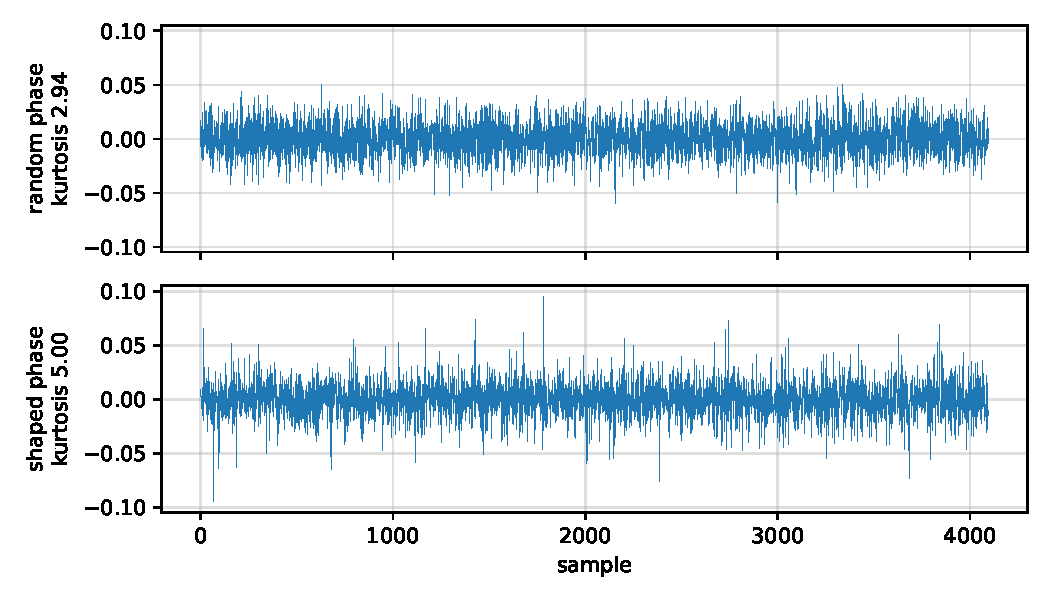
\includegraphics[width=0.85\textwidth]{figures/siso_block.pdf}
\caption{Identical flat magnitude spectrum, different phases. Top: random phases (Gaussian, kurtosis $2.94$). Bottom: shaped phases (kurtosis $5.00$).}
\label{fig:siso}
\end{figure}

\textbf{Convergence.} Figure~\ref{fig:convergence} shows the loss trajectory for the single-channel problem above, run to a stop value of $10^{-10}$: roughly $100$ objective evaluations, each costing a handful of FFTs. The spikes are rejected trial steps of the conservative CCSAQ outer loop.

\begin{figure}[htb]
\centering
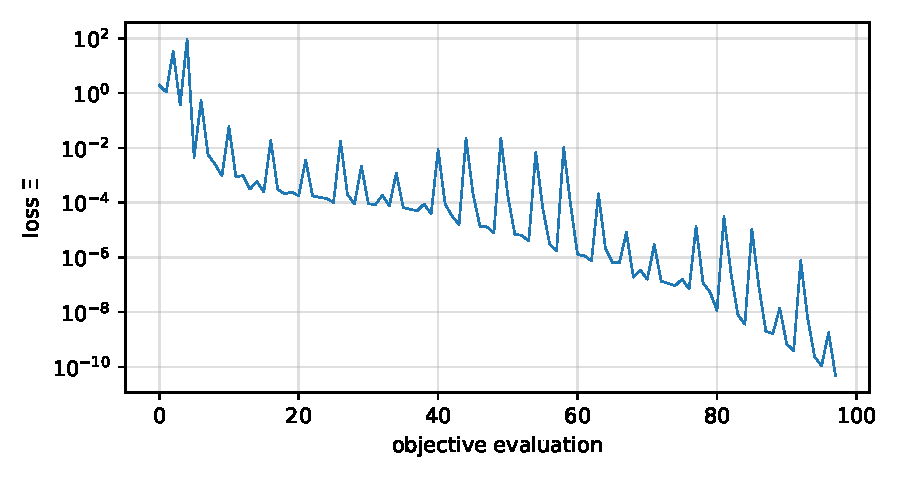
\includegraphics[width=0.7\textwidth]{figures/convergence.pdf}
\caption{Loss $\Xi$ versus objective evaluation for the single-channel kurtosis problem (CCSAQ, analytic gradients).}
\label{fig:convergence}
\end{figure}

\textbf{Minimum crest factor.} Figure~\ref{fig:crest} shows the crest surrogate of the previous section at work on the flat-spectrum single-channel problem ($N_t = 4096$), for the full band and for a half-band spectrum with a zero upper tail. The $\beta$-continuation (doubling from $5$ to $320$, warm-started) reaches a sampled crest factor of ${\approx}1.14$ for the full band and ${\approx}1.33$ for the half band, consistently across random seeds; direct single-stage runs at high $\beta$ plateau near $1.16$ despite several times the iteration budget. Two observations are worth recording. First, minimum crest and minimum kurtosis are \emph{different} signals: the crest-optimal blocks settle at kurtosis ${\approx}1.17$, visibly above the minimum achievable kurtosis of ${\approx}1.12$ for the same spectrum. Second, the sub-$\sqrt{2}$ full-band value must be read with the logical-versus-physical caveat of the previous section: near-Nyquist content allows the sample grid to sidestep the continuous waveform's peaks, so part of the margin below $\sqrt{2}$ is a discrete-sampling artefact. The half-band figure of $1.33$ is free of this effect and is the number relevant to a physical drive signal; the resulting waveform is a constant-envelope, noise-like block with no visible chirp structure.

\begin{figure}[htb]
\centering
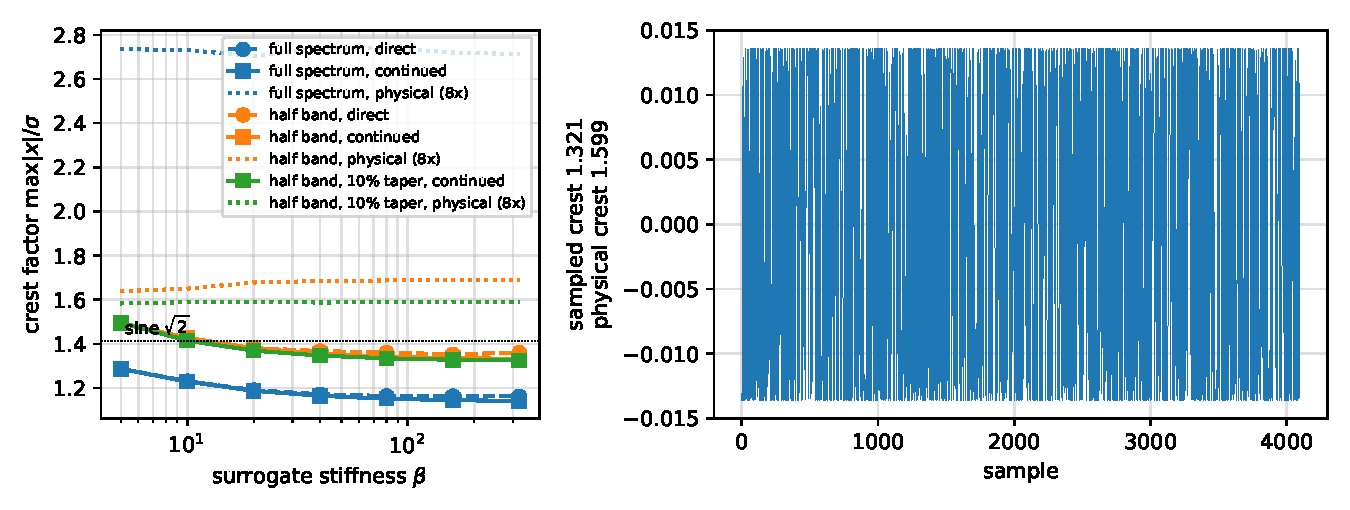
\includegraphics[width=0.95\textwidth]{figures/crest_beta.pdf}
\caption{Crest-factor minimisation with the logcosh surrogate. Left: achieved crest versus surrogate stiffness $\beta$, seed-averaged; warm-started $\beta$-continuation (solid) versus direct single-stage runs (dashed), for the full-band and half-band flat spectra. Right: the resulting full-band minimum-crest block.}
\label{fig:crest}
\end{figure}

\textbf{MIMO with measured targets.} A two-channel surrogate record is synthesised as coloured, correlated, non-Gaussian noise: channel $0$ is low-pass weighted and memorylessly distorted (skewed, heavy-tailed); channel $1$ shares a common source with channel $0$ through a resonance at $0.2\,f_s$. Targets are estimated per the previous section: multitaper CSD ($NW = 4$, $K = 7$ tapers, $16$ segments of $1024$ samples) factored per bin by Cholesky, and sample moments for the tuple set $\seq{(0,0,0),\,(1,1,1),\,(0,0,0,0),\,(1,1,1,1),\,(0,0,1,1)}$. Table~\ref{tab:mimo} lists targets and block-averaged achieved values over $32$ independently optimised blocks; Figure~\ref{fig:mimotraces} shows one synthesised block, and Figure~\ref{fig:csd} compares the target CSD with a multitaper estimate over the ensemble of synthesised blocks. PSD, coherence and cross phase are all reproduced. Estimating both sides with the same estimator matters here: per block the off-diagonal cross-spectrum is a single rank-one sample that carries a random phase factor $\m{e}^{\m{i}\mat{\psi_{0f}-\psi_{1f}}}$, so only the ensemble converges -- and at the low coherence of this record the phase scatter of a low-degrees-of-freedom estimate is large, of order $\sqrt{\mat{1/\gamma^2-1}/2N}$.

\begin{table}[htb]
\centering
\begin{tabular}{l l r r}
target & tuple $\mathbf{i}$ & $\mu_\mathbf{i}$ & achieved (mean $\pm$ std) \\
\hline
skewness ch.\,0 & $(0,0,0)$ & 3.081 & 3.067 $\pm$ 0.012 \\
skewness ch.\,1 & $(1,1,1)$ & -0.004 & -0.005 $\pm$ 0.005 \\
kurtosis ch.\,0 & $(0,0,0,0)$ & 17.246 & 17.246 $\pm$ 0.006 \\
kurtosis ch.\,1 & $(1,1,1,1)$ & 2.939 & 2.940 $\pm$ 0.005 \\
co-kurtosis $(0,0,1,1)$ & $(0,0,1,1)$ & 1.314 & 1.315 $\pm$ 0.003 \\
\end{tabular}

\caption{Measured-target MIMO example: moment targets estimated from the record versus block-averaged achieved values ($32$ blocks, $N_t = 1024$).}
\label{tab:mimo}
\end{table}

\begin{figure}[htb]
\centering
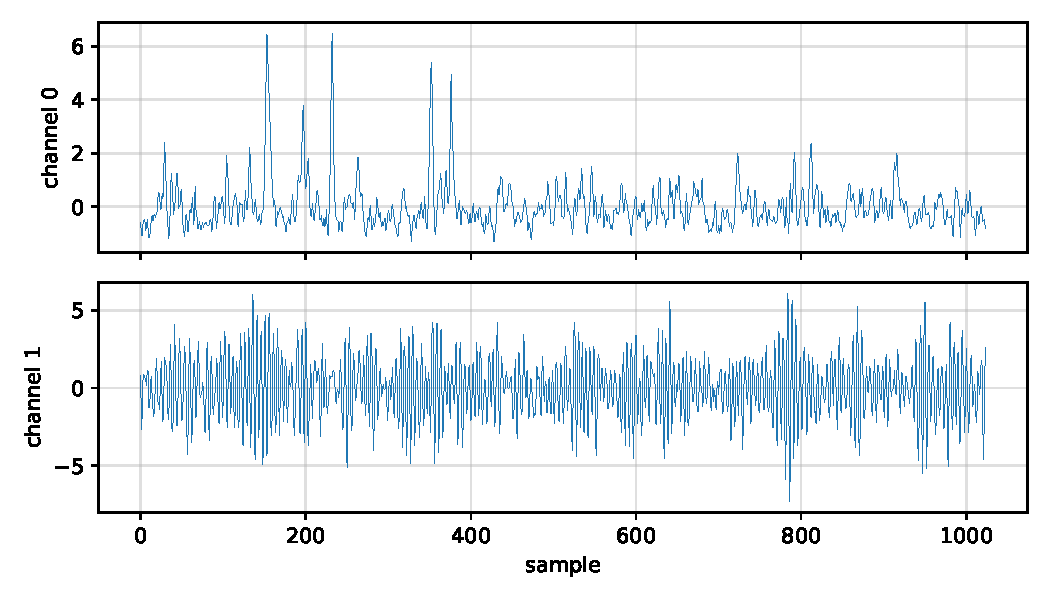
\includegraphics[width=0.85\textwidth]{figures/mimo_traces.pdf}
\caption{One synthesised MIMO block. Channel $0$ reproduces the strong skew and kurtosis of the record; channel $1$ stays near-Gaussian, as its targets dictate.}
\label{fig:mimotraces}
\end{figure}

\begin{figure}[htb]
\centering
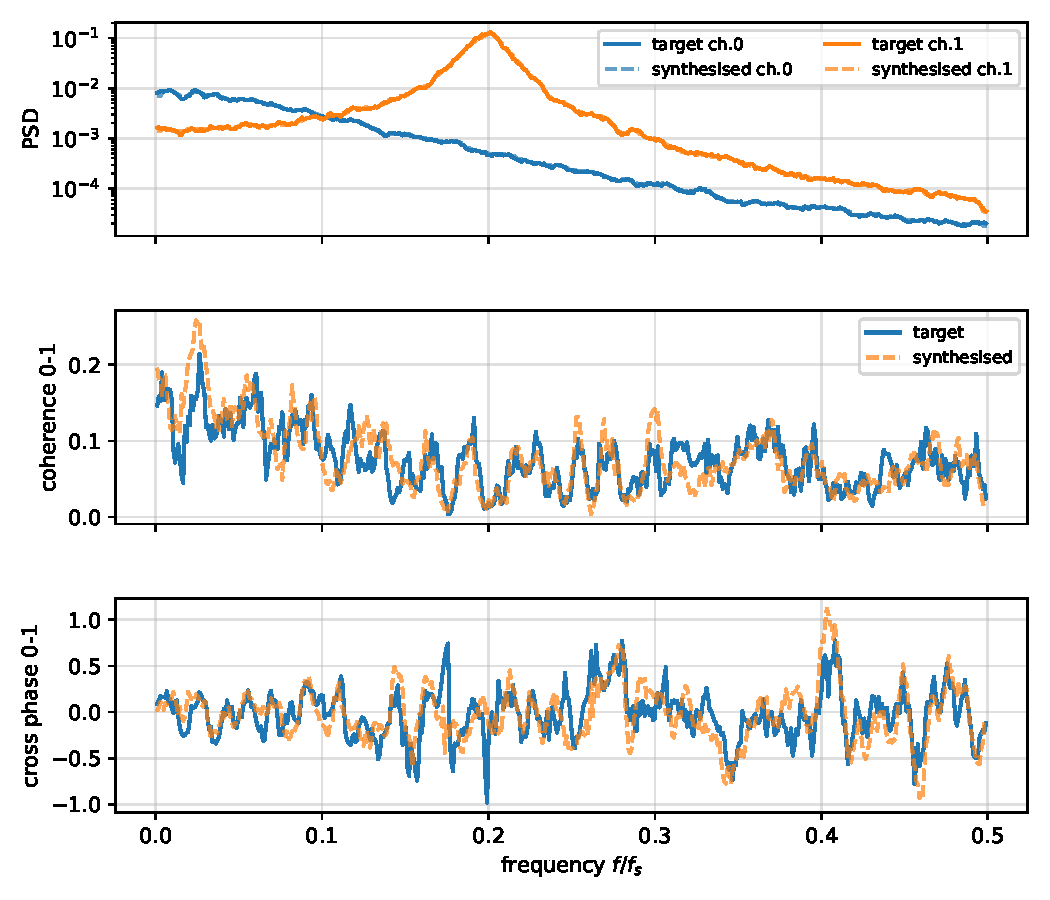
\includegraphics[width=0.85\textwidth]{figures/csd_match.pdf}
\caption{Target CSD versus a multitaper estimate over $32$ shaped blocks: PSD per channel (top), coherence (middle) and cross phase (bottom).}
\label{fig:csd}
\end{figure}

%=============================================================================================================================
\bibliography{refs}
%=============================================================================================================================

\end{document}
